\documentclass[letterpaper]{article}

\usepackage{gensymb}
\usepackage[vmargin=1in,hmargin=1.25in]{geometry}
\usepackage{graphicx}
\usepackage{hyperref}
\usepackage{microtype}
\usepackage{lmodern}

\author{Philip Pham}
\title{\Large ECE/CSE 576, Spring 2019 Homework 2: Creating Panoramas}
\date{\today}

\begin{document}
\maketitle

\section{Harris Corner Detector}
\label{sec:harris}
Gaussian blurring was applied with $\sigma = 2$. The Harris response threshold
was $50$, and non-maximal suppression was done with a $5 \times 5$
window. Detected corners are denoted with a red cross. As a sanity check, we
apply the algorithm to \texttt{Boxes.png}.

\begin{center}
  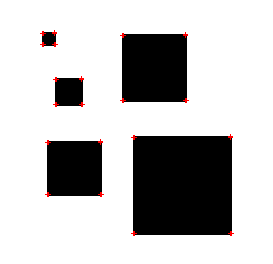
\includegraphics{1a.png}  
\end{center}

\begin{center}
  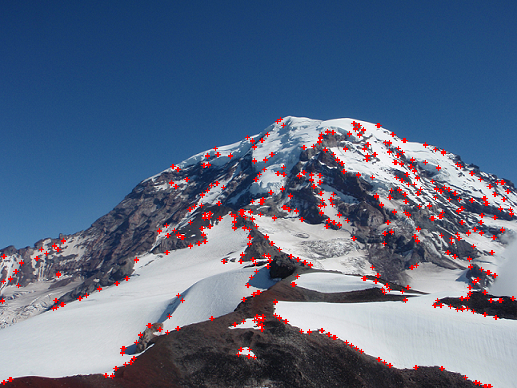
\includegraphics[width=0.73\textwidth]{1b.png}
  
  Applied to \texttt{Rainier1.png}.
\end{center}

\begin{center}
  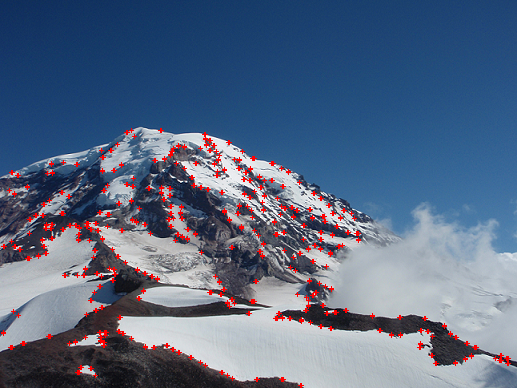
\includegraphics[width=0.73\textwidth]{1c.png}
  
  Applied to \texttt{Rainier2.png}.
\end{center}

\section{Match Corner Points}

The $l_1$ norm applied to the feature descriptor was used to find matching
corner points in the other image.

\begin{center}
  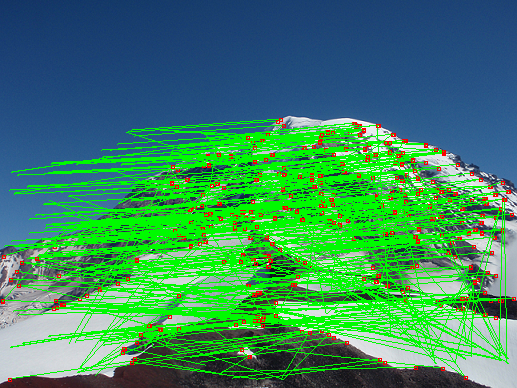
\includegraphics[width=0.85\textwidth]{2a.png}
  
  All matching corner points in \texttt{Rainier1.png}.
\end{center}

\begin{center}
  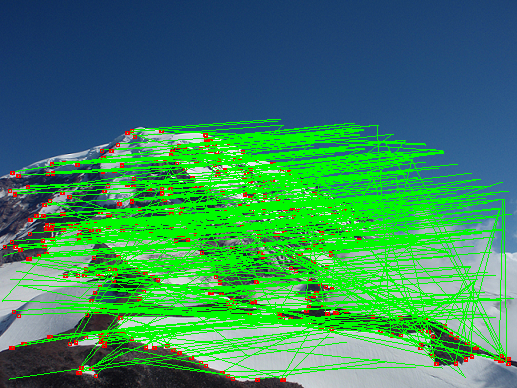
\includegraphics[width=0.85\textwidth]{2b.png}
  
  All matching corner points in \texttt{Rainier2.png}.
\end{center}

\section{RANSAC}

Homographies were sampled by choosing 4 matches. The homography with the largest
number of inliers was chosen.

\begin{center}
  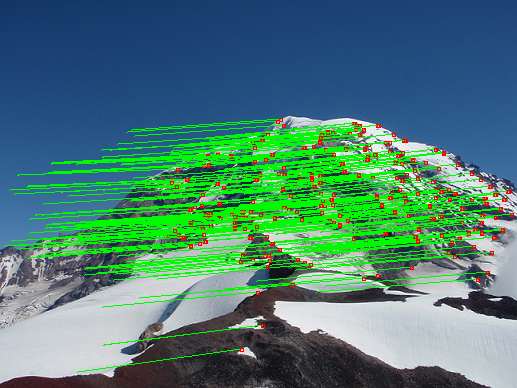
\includegraphics[width=0.85\textwidth]{3a.png}
  
  Matches from the homography with the largest number of inliers in
  \texttt{Rainier1.png}.
\end{center}

\begin{center}
  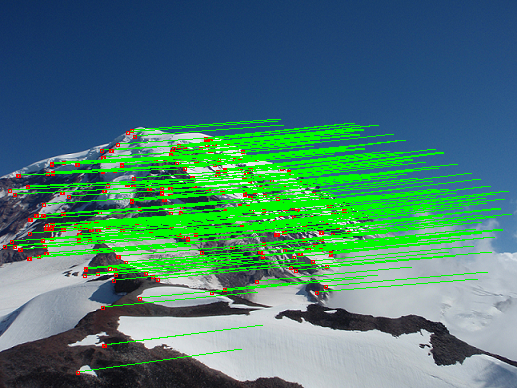
\includegraphics[width=0.85\textwidth]{3b.png}
  
  Matches from the homography with the largest number of inliers in
  \texttt{Rainier2.png}.
\end{center}

\section{Stitch}
\label{sec:stitch}

A flat panorama was made by using the first image as the reference coordinate
system.

\begin{center}
  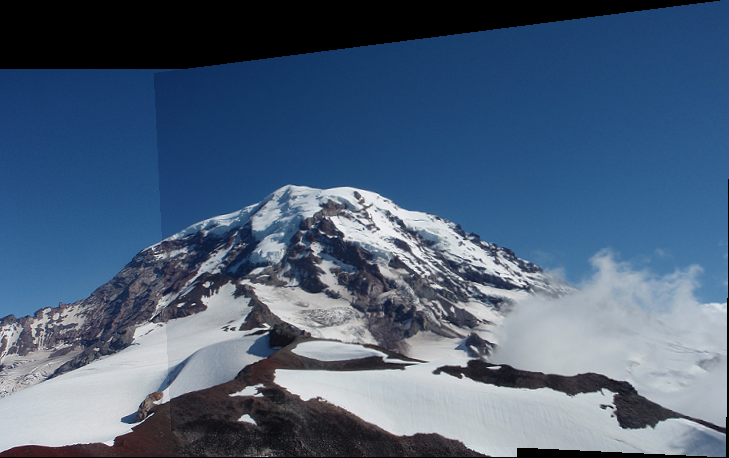
\includegraphics[width=0.9\textwidth]{4.png}
  
  The result of stitching \texttt{Ranier1.png} and \texttt{Ranier2.png}.
\end{center}

\section*{Bell: Complete Mt. Ranier Panorama}

The same technique in Section \ref{sec:stitch} can be applied repeatedly to get a
complete panorama.

\begin{center}
  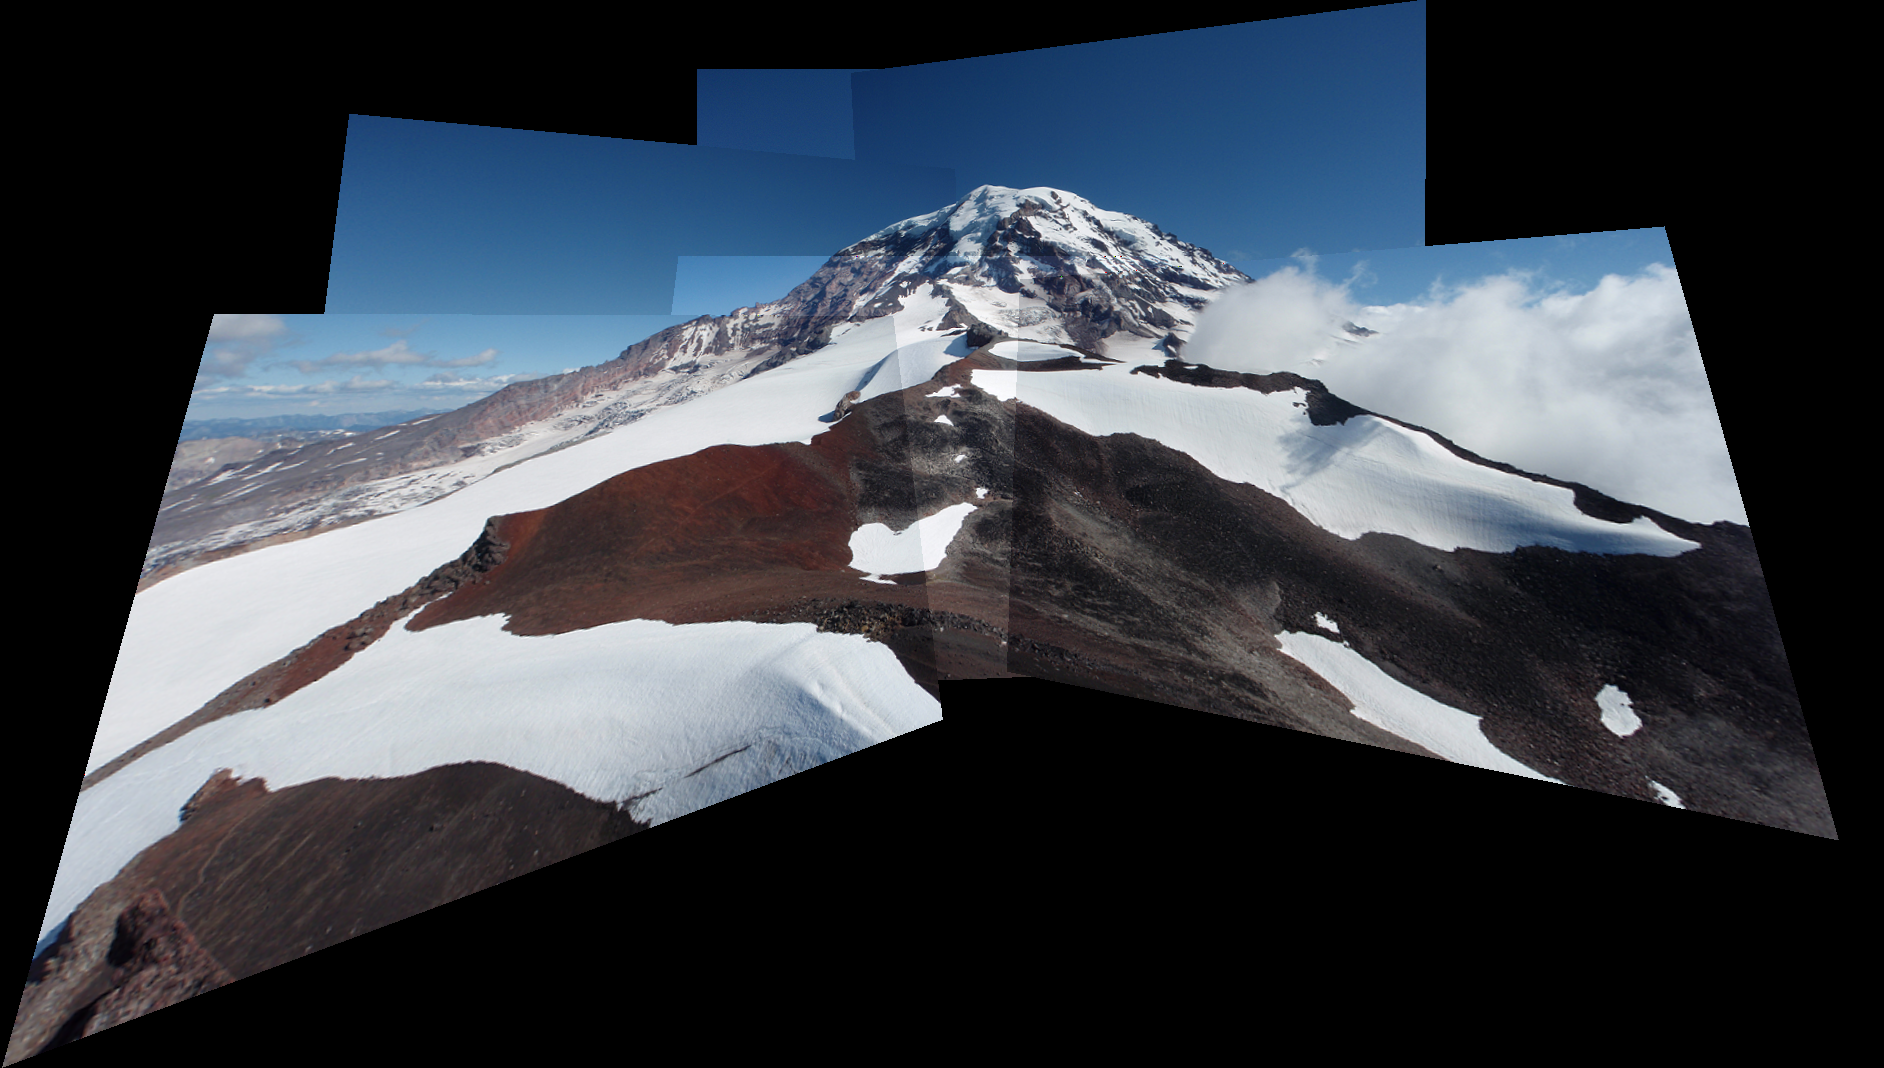
\includegraphics[width=\textwidth]{all_stitched.png}
  
  The result of stitching \texttt{Ranier1.png}, \texttt{Ranier2.png},
  \texttt{Ranier3.png}, \texttt{Ranier4.png}, \texttt{Ranier5.png}, and
  \texttt{Ranier6.png}.
\end{center}

\section*{Whistle: Center-weighting}

In Section \ref{sec:stitch} the seam between the two stitched images is
apparent. Center-weighting can be used to make seam invisible.

\begin{center}
  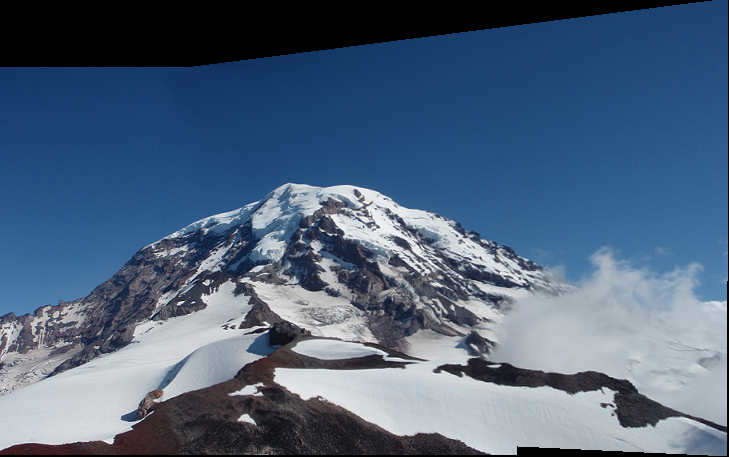
\includegraphics[width=0.9\textwidth]{4_center_weighted.png}
  
  The result of stitching \texttt{Ranier1.png} and \texttt{Ranier2.png} with
  center-weighting.
\end{center}

The same can be done with the complete panorama.

\begin{center}
  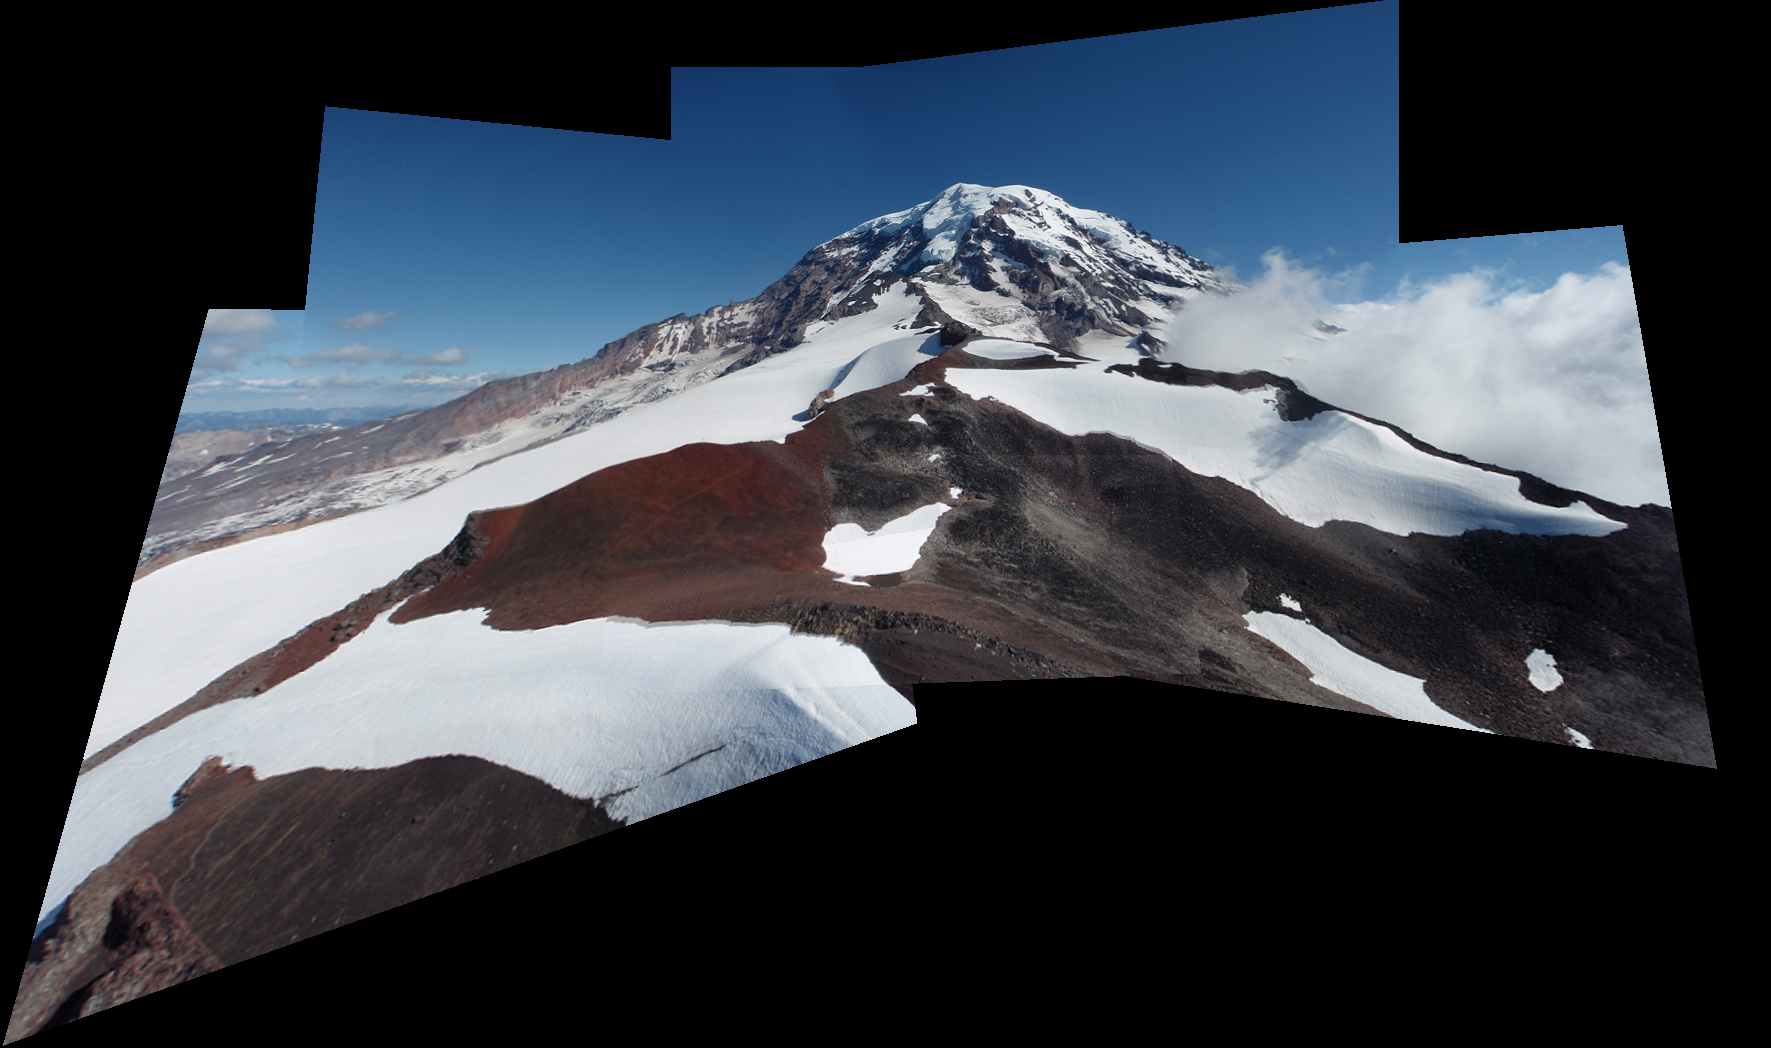
\includegraphics[width=\textwidth]{all_stitched_center_weighted.png}
  
  The result of stitching \texttt{Ranier1.png}, \texttt{Ranier2.png},
  \texttt{Ranier3.png}, \texttt{Ranier4.png}, \texttt{Ranier5.png}, and
  \texttt{Ranier6.png} with center-weighting.
\end{center}


\end{document}
